\chapter{Simulation of quantum algorithms in a memory-efficient way}

In this chapter I will examine the architecture and implementation of the framework that is capable of running simulations of gated general-purpose quantum computation.

\section{Design goals}

For an $n$ qubit register, the register itself must be stored using $2^n$ complex numbers (the probability amplitudes of each of the $2^n$ 0/1 variations), however the size of the matrix that is applied to it is $(2^n)^2$, which is considerably larger.

Qiskit uses a lot of memory, because it stores every single quantum operator matrix in memory. Furhermore, even if the operation is the same, if it is applied multiple times, individual instances of the matrix are created. This is extremely wasteful.

While it uses some techniques to reduce the memory allocations, such as sparse matrix representation, this cannot fundamentally get around the issue, that the architecture itself does not allow flexibility of operator representation.

Instead of storing the matrices in-memory I will be designing a system where operators can be created without the need for a matrix representation at all, or when that is not possible the currently used column of the matrix can be generated "on-the-fly" for application.

\section{Quantum registers}

The first step in the implementation process is designing the inner workings of the quantum registers. In order to represent an $n$ qubit register, we must store $2^n$ complex numbers, the probability amplitudes of each of the possible 0/1 bit representations.

\begin{align*}
\ket{0\dots{}000} \rightarrow & \hspace{2mm} c_0 \\
\ket{0\dots{}001} \rightarrow & \hspace{2mm}  c_1 \\
\ket{0\dots{}010} \rightarrow & \hspace{2mm} c_2 \\
\ket{0\dots{}011} \rightarrow & \hspace{2mm} c_3 \\
\dots{} \\
\ket{1\dots{}111} \rightarrow & \hspace{2mm} c_{2^n-1}
\end{align*}

Where $c_0,\dots{},c_{2^n-1}\in{}\mathds{C}$.

When multiple registers are present in the system, handling operators that are only applied to some of the registers becomes problematic. Since qubits can be entangled, every single new register added to the system multiplies the amount of storage required for the probability amplitudes.

\subsection{General solution}

Let there be $r$ registers in the system: 

\begin{align*}
\{R_0, \dots{}, R_{r-1}\}
\end{align*}

and let $n_i$ be number of qubits in register $R_i$, where $(0\leq{}i<r)$.

The total number of qubits in the system is therefore

\begin{align*}
    n = \sum\limits_{i=0}^{r-1}n_{i}.
\end{align*}

Then, let $U$ be an operation, a unitary (square) matrix, that is applied to $k$ of the registers:

\begin{align*}
\{R_{r_0},\dots{},R_{r_{k-1}}\},\hspace{3mm} (0\leq{}r_j<r),\hspace{3mm} (0\leq{}j<k),\hspace{3mm} (k\leq{}r).
\end{align*}

The number of qubits $U$ must operate on is therefore

\begin{align*}
    m = \sum\limits_{j=0}^{k-1}l_{r_j}.
\end{align*}

which means that the $U$ matrix is of size $(M\times{}M)$, where

\begin{align*}
M = 2^m = \prod\limits_{j=0}^{k-1} 2^{(l_{r_j})}.
\end{align*}

The complex probability amplitudes for all possible register contents in the system are stored in a single array $C$, of complex numbers. $C$'s size is 

\begin{align*}
N = 2^n = \prod\limits_{i=0}^{r-1} 2^{l_i}.
\end{align*}

and its contents are

\begin{align*}
C = [C[0],\dots{},C[N-1]] \in{} \mathds{C}^N
\end{align*}

Let us introduce binary indexing sequences on $C$. A sequence of qubits

\begin{align*}
\ket{b_{n-1},b_{n-2},\dots{},b_2,b_1,b_0},
\end{align*}

is a binary indexing sequence on $C$ and it corresponds to

\begin{align*}
C[\ket{b_{n-1},b_{n-2},\dots{},b_2,b_1,b_0}] = C[B],
\end{align*}

where
\begin{align*}
B = \sum\limits_{i=0}^{n-1}b_i\cdot{}2^{i}.
\end{align*}

A binary indexing sequence is partitioned by the registers in the following way:

\begin{align*}
\ket{b_{n-1},b_{n-2},\dots{},b_2,b_1,b_0} = \ket{R_{r-1} | R_{r-2} | \dots{} | R_2 | R_1 | R_0}.
\end{align*}

Similarly, a single cell of the $U$ matrix can be indexed using 2-dimensional binary indexing sequences. The matrix $U$ is indexed by the following 2 $m$ dimensional qubit sequences:

\begin{align*}
\ket{a_{m-1},a_{n-2},\dots{},a_2,a_1,a_0}
\end{align*}

and

\begin{align*}
\ket{b_{m-1},b_{n-2},\dots{},b_2,b_1,b_0}.
\end{align*}

and it corresponds to

\begin{align*}
U[\ket{a_{m-1},a_{n-2},\dots{},a_2,a_1,a_0}][\ket{b_{m-1},b_{n-2},\dots{},b_2,b_1,b_0}] = U[A][B],
\end{align*}

where

\begin{align*}
A = \sum\limits_{i=0}^{n-1}a_i\cdot{}2^{i}
\end{align*}

and

\begin{align*}
B = \sum\limits_{i=0}^{n-1}b_i\cdot{}2^{i}.
\end{align*}

A 2-dimensional binary indexing sequence on the U matrix can also be partitioned by the registers $U$ is applied to, in the following ways:

\begin{align*}
\ket{a_{m-1},a_{m-2},\dots{},a_2,a_1,a_0} = \ket{R_{r_{k-1}} | R_{r_{k-2}} | \dots{} | R_{r_2} | R_{r_1} | R_{r_0}}.
\end{align*}

and

\begin{align*}
\ket{b_{m-1},b_{m-2},\dots{},b_2,b_1,b_0} = \ket{R_{r_{k-1}} | R_{r_{k-2}} | \dots{} | R_{r_2} | R_{r_1} | R_{r_0}}.
\end{align*}

To implement the application of the $U$ matrix to registers $\{R_{r_0},\dots{},R_{r_{k-1}}\}$ in the system, the $C$ array must be rearranged, so that $U$ can be applied to continuous subsequences of $C$.

This can be done via a bit-mapping on the binary indexing sequences. The qubits corresponding to the registers $\{R_{r_0},\dots{},R_{r_{k-1}}\}$ are moved to the lower end of the sequence, while the rest of the registers to the upper end.

Let us index the registers $U$ is not applied to with $\{s_0, \dots{}, s_{n-k-1}\}$, so that

\begin{align*}
\{0, \dots{}, n-1\} = \{r_0, \dots{}, r_{k-1}\} \dot{\cup} \{s_0, \dots{}, s_{n-k-1}\}. 
\end{align*}

Then, the binary index sequence mapping (BISM) is defined as

\begin{align*}
\text{\textbf{BISM}}: \ket{R_{r-1} | R_{r-2} | \dots{} | R_2 | R_1 | R_0} \rightarrow \ket{R_{s_{r-k-1}} | \dots{} | R_{s_0} \mathbf{|} R_{r_{k-1}} | \dots{} | R_{r_0} }.
\end{align*}

The \textbf{BISM} function can be used to define the permutation on the $C$ array, by mapping

\begin{align*}
C'[\text{\textbf{BISM}}(B)] = C[B], \hspace{3mm}(0\leq{}B<N).
\end{align*}

The $C'$ array's binary indexing sequences can now be partitioned into an upper and lower region,

\begin{align*}
\ket{b'_{n-1},\dots{},b'_{m}|b'_{m-1},\dots{}b'_0},
\end{align*}

where the lower region's indexing sequences correspond 1-to-1 to the $U$ unitary matrix operation's second dimension.

With everything set up, we can now define the application of $U$ to $C'$. Let the resulting register contents be $R'$, where

\begin{align}
\label{RowGenEq}
R'[\ket{b'_{n-1},\dots{},b'_{k}|a'_{k-1},\dots{}a'_0}] = \sum\limits_{\substack{0\leq{}i<m \\ \forall{}b_i\in{}\{0,1\}}}U[\ket{a'_{m-1},\dots{},a'_0}][\ket{b'_{m-1},\dots{},b'_0}] \cdot{} C'[\ket{b'_{m-1},\dots{},b'_0}].
\end{align}

During this application, we can see that the matrix is read in a column-by-column fashion, which means that we only need to generate a single column of $U$.

In cases where the operation is a mapping or aggregation itself (such as the WeightedAdder from the Grover's search), it can be performed without generating the column itself, the same permutation logic is used, but instead of generating an entire row of $U$, the $\ket{a'_{m-1},\dots{},a'_0}$ "output index" is calculated based on the $\ket{b'_{m-1},\dots{},b'_0}$ "input index" by a function

\begin{align*}
    u: \ket{b'_{m-1},\dots{},b'_0} \rightarrow \ket{a'_{m-1},\dots{},a'_0},
\end{align*}

which then replaces the matrix multiplication as follows:

\begin{align}
\label{NoGenEq}
R'[\ket{b'_{n-1},\dots{},b'_{k}|a'_{k-1},\dots{}a'_0}] =
\sum\limits_{\substack{0\leq{}i<m \\ \forall{}b_i\in{}\{0,1\}\\ u(\ket{b'_{m-1},\dots{},b'_0}) =
\ket{a'_{m-1},\dots{},a'_0}}}C'[\ket{b'_{m-1},\dots{},b'_0}].
\end{align}

These equations are the basis of the memory-efficiency of this framework.

Finally, the $R'$ array must be inverse-permuted back to the original order of the indexing qubits

\begin{align*}
R[B] = R'[\text{\textbf{BISM}}(B)], \hspace{3mm}(0\leq{}B<N).
\end{align*}

\subsection{Presenting the solution on an example}

For example when 3 registers are present, $R_0$ consisting of $1$ qubit, $R_1$ consisting of $1$ qubits and $R_2$ consisting of $2$ qubits, then the binary indexing sequence of the amplitude registers is the following: $\ket{R_{2,0},R_{2,1};R_{1,0};R_{0,0}}$.

The probability amplitudes stored are the following:
\begin{align*}
\ket{00,0,0} \rightarrow & \hspace{2mm} c_{0} &
\ket{10,0,0} \rightarrow & \hspace{2mm} c_{8} \\
\ket{00,0,1} \rightarrow & \hspace{2mm} c_{1} &
\ket{10,0,1} \rightarrow & \hspace{2mm} c_{9} \\
\ket{00,1,0} \rightarrow & \hspace{2mm} c_{2} &
\ket{10,1,0} \rightarrow & \hspace{2mm} c_{10} \\
\ket{00,1,1} \rightarrow & \hspace{2mm} c_{3} &
\ket{10,1,1} \rightarrow & \hspace{2mm} c_{11} \\
\\
\ket{01,0,0} \rightarrow & \hspace{2mm} c_{4} &
\ket{11,0,0} \rightarrow & \hspace{2mm} c_{12} \\
\ket{01,0,1} \rightarrow & \hspace{2mm} c_{5} &
\ket{11,0,1} \rightarrow & \hspace{2mm} c_{13} \\
\ket{01,1,0} \rightarrow & \hspace{2mm} c_{6} &
\ket{11,1,0} \rightarrow & \hspace{2mm} c_{14} \\
\ket{01,1,1} \rightarrow & \hspace{2mm} c_{7} &
\ket{11,1,1} \rightarrow & \hspace{2mm} c_{15} \\
\end{align*}

The simplest solution would be to apply a "no-operation" operator, or the identity matrix to the remaining registers, however this will not scale well memory-wise with the number of registers increasing in the system.

Instead I implemented the register handling in a way that allowed me to skip storing "no-operation" matrices in the memory completely. In order to apply an operator to only some registers in the system, the probability amplitudes are re-arranged in a way so that a continuous section of memory corresponds to a column of the matrix. This way, the matrix operation can be applied to sections of probability amplitudes iteratively.

For example, if we apply a $3$ qubit operator to the registers $R_0$ and $R_2$, then the previous table is rearranged so that the bits corresponding to $R_0$ and $R_2$ are pushed towards the least significant bit in the following way:

\begin{align*}
\ket{R_{2,1},R_{2,1};R_{1,0};R_{0,0}} \rightarrow \ket{R_{1,0};\color{red}R_{2,0},R_{2,1};R_{0,0}\color{black}}
\end{align*}


\begin{align*}
\ket{00,0,0} \rightarrow & \ket{0,\color{red}00,0\color{black}}' \rightarrow \color{red}c'_{0}\color{black}\rightarrow c_{0} &
\ket{10,0,0} \rightarrow & \ket{0,\color{red}10,0\color{black}}' \rightarrow \color{red}c'_{4}\color{black}\rightarrow c_{8} \\
\ket{00,0,1} \rightarrow & \ket{0,\color{red}00,1\color{black}}' \rightarrow \color{red}c'_{1}\color{black}\rightarrow c_{1} &
\ket{10,0,1} \rightarrow & \ket{0,\color{red}10,1\color{black}}' \rightarrow \color{red}c'_{5}\color{black}\rightarrow c_{9} \\
\ket{00,1,0} \rightarrow & \ket{1,\color{red}00,0\color{black}}' \rightarrow \color{red}c'_{8}\color{black}\rightarrow c_{2} &
\ket{10,1,0} \rightarrow & \ket{1,\color{red}10,0\color{black}}' \rightarrow \color{red}c'_{12}\color{black}\rightarrow c_{10} \\
\ket{00,1,1} \rightarrow & \ket{1,\color{red}00,1\color{black}}' \rightarrow \color{red}c'_{9}\color{black}\rightarrow c_{3} &
\ket{10,1,1} \rightarrow & \ket{1,\color{red}10,1\color{black}}' \rightarrow \color{red}c'_{13}\color{black}\rightarrow c_{11} \\
\\
\ket{01,0,0} \rightarrow & \ket{0,\color{red}01,0\color{black}}' \rightarrow \color{red}c'_{2}\color{black}\rightarrow c_{4} &
\ket{11,0,0} \rightarrow & \ket{0,\color{red}11,0\color{black}}' \rightarrow \color{red}c'_{6}\color{black}\rightarrow c_{12} \\
\ket{01,0,1} \rightarrow & \ket{0,\color{red}01,1\color{black}}' \rightarrow \color{red}c'_{3}\color{black}\rightarrow c_{5} &
\ket{11,0,1} \rightarrow & \ket{0,\color{red}11,1\color{black}}' \rightarrow \color{red}c'_{7}\color{black}\rightarrow c_{13} \\
\ket{01,1,0} \rightarrow & \ket{1,\color{red}01,0\color{black}}' \rightarrow \color{red}c'_{10}\color{black}\rightarrow c_{6} &
\ket{11,1,0} \rightarrow & \ket{1,\color{red}11,0\color{black}}' \rightarrow \color{red}c'_{14}\color{black}\rightarrow c_{14} \\
\ket{01,1,1} \rightarrow & \ket{1,\color{red}01,1\color{black}}' \rightarrow \color{red}c'_{11}\color{black}\rightarrow c_{7} &
\ket{11,1,1} \rightarrow & \ket{1,\color{red}11,1\color{black}}' \rightarrow \color{red}c'_{15}\color{black}\rightarrow c_{15} \\
\end{align*}

Then, the 3 qubit operator $U^{8\times{}8}$, which is an $(8\times8)$ matrix can be applied iteratively in the following way:

\begin{enumerate}
    \item Apply $U^{8\times{}8}$ to the probability amplitudes corresponding to $R_{1,0} = \ket{0}$\\
    $[c_0,c_1,c_4,c_5,c_8,c_9,c_{12},c_{13}] = [\color{red}c'_0,c'_1,c'_2,c'_3,c'_4,c'_5,c'_6,c'_7\color{black}]$\\
    The resulting vector is the first half of the complete result:\\
    $[\color{red}r'_0,r'_1,r'_2,r'_3,r'_4,r'_5,r'_6,r'_7\color{black}]$
    \item Apply $U^{8\times{}8}$ to the probability amplitudes corresponding to $R_{1,0} = \ket{1}$\\
    $[c_2,c_3,c_6,c_7,c_{10},c_{11},c_{14},c_{15}] = [\color{red}c'_8,c'_9,c'_{10},c'_{11},c'_{12},c'_{13},c'_{14},c'_{15}\color{black}]$\\
    The resulting vector is the second half of the complete result:\\
    $[\color{red}r'_8,r'_9,r'_{10},r'_{11},r'_{12},r'_{13},r'_{14},r'_{15}\color{black}]$
    \item Iterate over all values for the untouched register $R_1$ and aggregate the results:\\
     $[\color{red}r'_0,r'_1,r'_2,r'_3,r'_4,r'_5,r'_6,r'_7,r'_8,r'_9,r'_{10},r'_{11},r'_{12},r'_{13},r'_{14},r'_{15}\color{black}]$.
    \item Revert the mapping to the original indexes:\\ $[\color{red}r'_0,r'_1,r'_2,r'_3,r'_4,r'_5,r'_6,r'_7,r'_8,r'_9,r'_{10},r'_{11},r'_{12},r'_{13},r'_{14},r'_{15}\color{black}] =$\\
    $[r_0,r_1,r_4,r_5,r_8,r_9,r_{12},r_{13},r_2,r_3,r_6,r_7,r_{10},r_{11},r_{14},r_{15}]$.
\end{enumerate}

\section{Quantum operators}

In order to implement Grover's algorithm the following operators are needed: Hadamard, Grover (Diffuser matrix), Sum (WeightedAdder), and Multi-Controlled NOT.

\subsection{Definitions}

\subsubsection{Hadamard}

The Hadamard matrix is defined as follows. First, the $(2\times{}2)$ H matrix is the following:

\begin{align*}
  \mathbf{H} = \frac{1}{\sqrt{2}}\begin{pmatrix}
      1 & 1  \\
      1 & -1
    \end{pmatrix}.
\end{align*}

A $(2^n\times{}2^n)$ dimensional Hadamard matrix can be created by taking the tensor product of the $(2\times{}2)$ H matrix $n$ times: $\mathbf{H}^{\otimes{}n}$.

From this equation the $j$th column of the $i$th row of the $(2^n\times{}2^n)$ matrix can be defined by taking the \textbf{BITWISE\_AND} between the $i$ and $j$ indexes in binary form, then counting the set bits in that selector, to decide which cells should get a negative multiplier, as follows:

\newcommand*\circled[1]{\tikz[baseline=(char.base)]{
            \node[shape=circle,draw,inner sep=1pt] (char) {#1};}}

\begin{align*}
H[i][j] = \frac{1}{\sqrt{2^n}}\cdot{}(-1)^{\text{\textbf{COUNT\_BITS}}(i_{\text{\circled{2}}} \text{\textbf{ BITWISE\_AND }} j_{\text{\circled{2}}})}.
\end{align*}

This equation is directly implemented and a single column of $H$ is generated on-the-fly when $H$ is applied, using equation (\ref{RowGenEq}).

\subsubsection{Grover}

The Grover matrix is the diffusion operator from Grover's algorithm. It is defined using the $\mathbf{H}^{\otimes{}n}$ matrix, as follows.

Let's define the register $\ket{D}$ to be the following:

\begin{align*}
\ket{D} = \mathbf{H}^{\otimes{}n}\ket{0} =
\frac{1}{\sqrt{2^n}} \sum\limits_{i=0}^{2^n-1} \ket{i}.
\end{align*}

Then $G$ is the following matrix:

\begin{align*}
    \mathbf{G} = 2\ket{D}\bra{D} - \mathbf{I}.
\end{align*}

If $N = 2^n$, then $\mathbf{G}$ can be represented as follows:

\begin{align*}
  \mathbf{G} = \begin{pmatrix}
      \frac{2}{N} - 1 & \frac{2}{N} & \dots  & \frac{2}{N} \\
      \frac{2}{N} & \frac{2}{N} - 1 & \dots  & \frac{2}{N} \\
      \vdots & \vdots & \ddots & \vdots \\
      \frac{2}{N} & \frac{2}{N} & \ddots & \frac{2}{N} - 1
    \end{pmatrix}.
\end{align*}

It is straightforward to implement $G$, since the the $j$th column is $\frac{2}{N}$, except for the $j$th cell, where it is $\frac{2}{N}-1$. This matrix is also generated on-the-fly, column-by-column, using equation (\ref{RowGenEq}).

\subsubsection{Sum}

The sum operator is one, that can be represented directly using equation (\ref{NoGenEq}), by defining the

\begin{align*}
    u: \ket{b_{m-1},\dots{},b_0} \rightarrow \ket{a_{m-1},\dots{},a_0}
\end{align*}

function.

First, the $m$ qubits of the opetor are partitioned into two parts: input and output

\begin{align*}
m = s + \ceil{\log_{2}(s)},
\end{align*}

since the sum of $s$ qubits can be represented on $\ceil{\log_{2}(s)}$ bits.

Then, $u$ is defined as 

\begin{align*}
    u: \ket{0,\dots{},0,b_{s-1}\dots{},b_0} \rightarrow \ket{\text{\textbf{COUNT\_BITS}}(b_{s-1}\dots{},b_0),b_{s-1}\dots{},b_0}.
\end{align*}

\subsubsection{Multi-controlled NOT}

Similarly to \textbf{Sum}, a Multi-controlled NOT operator is defined using an $u$ function, which applies the $NOT$ operator to its most significant bit, when any of the other bits are set.

\begin{align*}
    u: \ket{b_{m-1},b_{m-2}\dots{},b_0} \rightarrow \ket{(\vee(b_{m-2}\dots{},b_0) \oplus{} b_{m-1}),b_{m-2}\dots{},b_0}.
\end{align*}

\section{Implementation and design patterns}

The goal of this framework is to allow the user to define quantum operators in a memory-efficient way. There are two types of operators: the ones that are columnwise generated on-the-fly and the $u$ function operators, directly interacting with the binary indexing sequences of the registers.

The code for register handling, the \textbf{BISM} operator and the permutation of the probability amplitudes is common amongst all operators. When these operators are being used, they must be callable from the same interface, to ensure that they are interchangeable and can be inherited from.

In order to achieve this, I have implemented the Strategy design pattern. The intent of this pattern, according to the Design Patters\cite{DesignPatterns} book is to define a family of algorithms, encapsulate each one, and make them interchangeable. Strategy lets the algorithm vary independently from clients that use it. In this pattern, a common interface is defined for all operators, with the implementation dependent on the specific operator. This common interface will later allow me to pontentially generate circuit diagrams for an implemented quantum algorithm.

In the UML diagram below, we can see the part of the system that deals with these memory-efficient operators.

\begin{figure}[H]
    \centering
    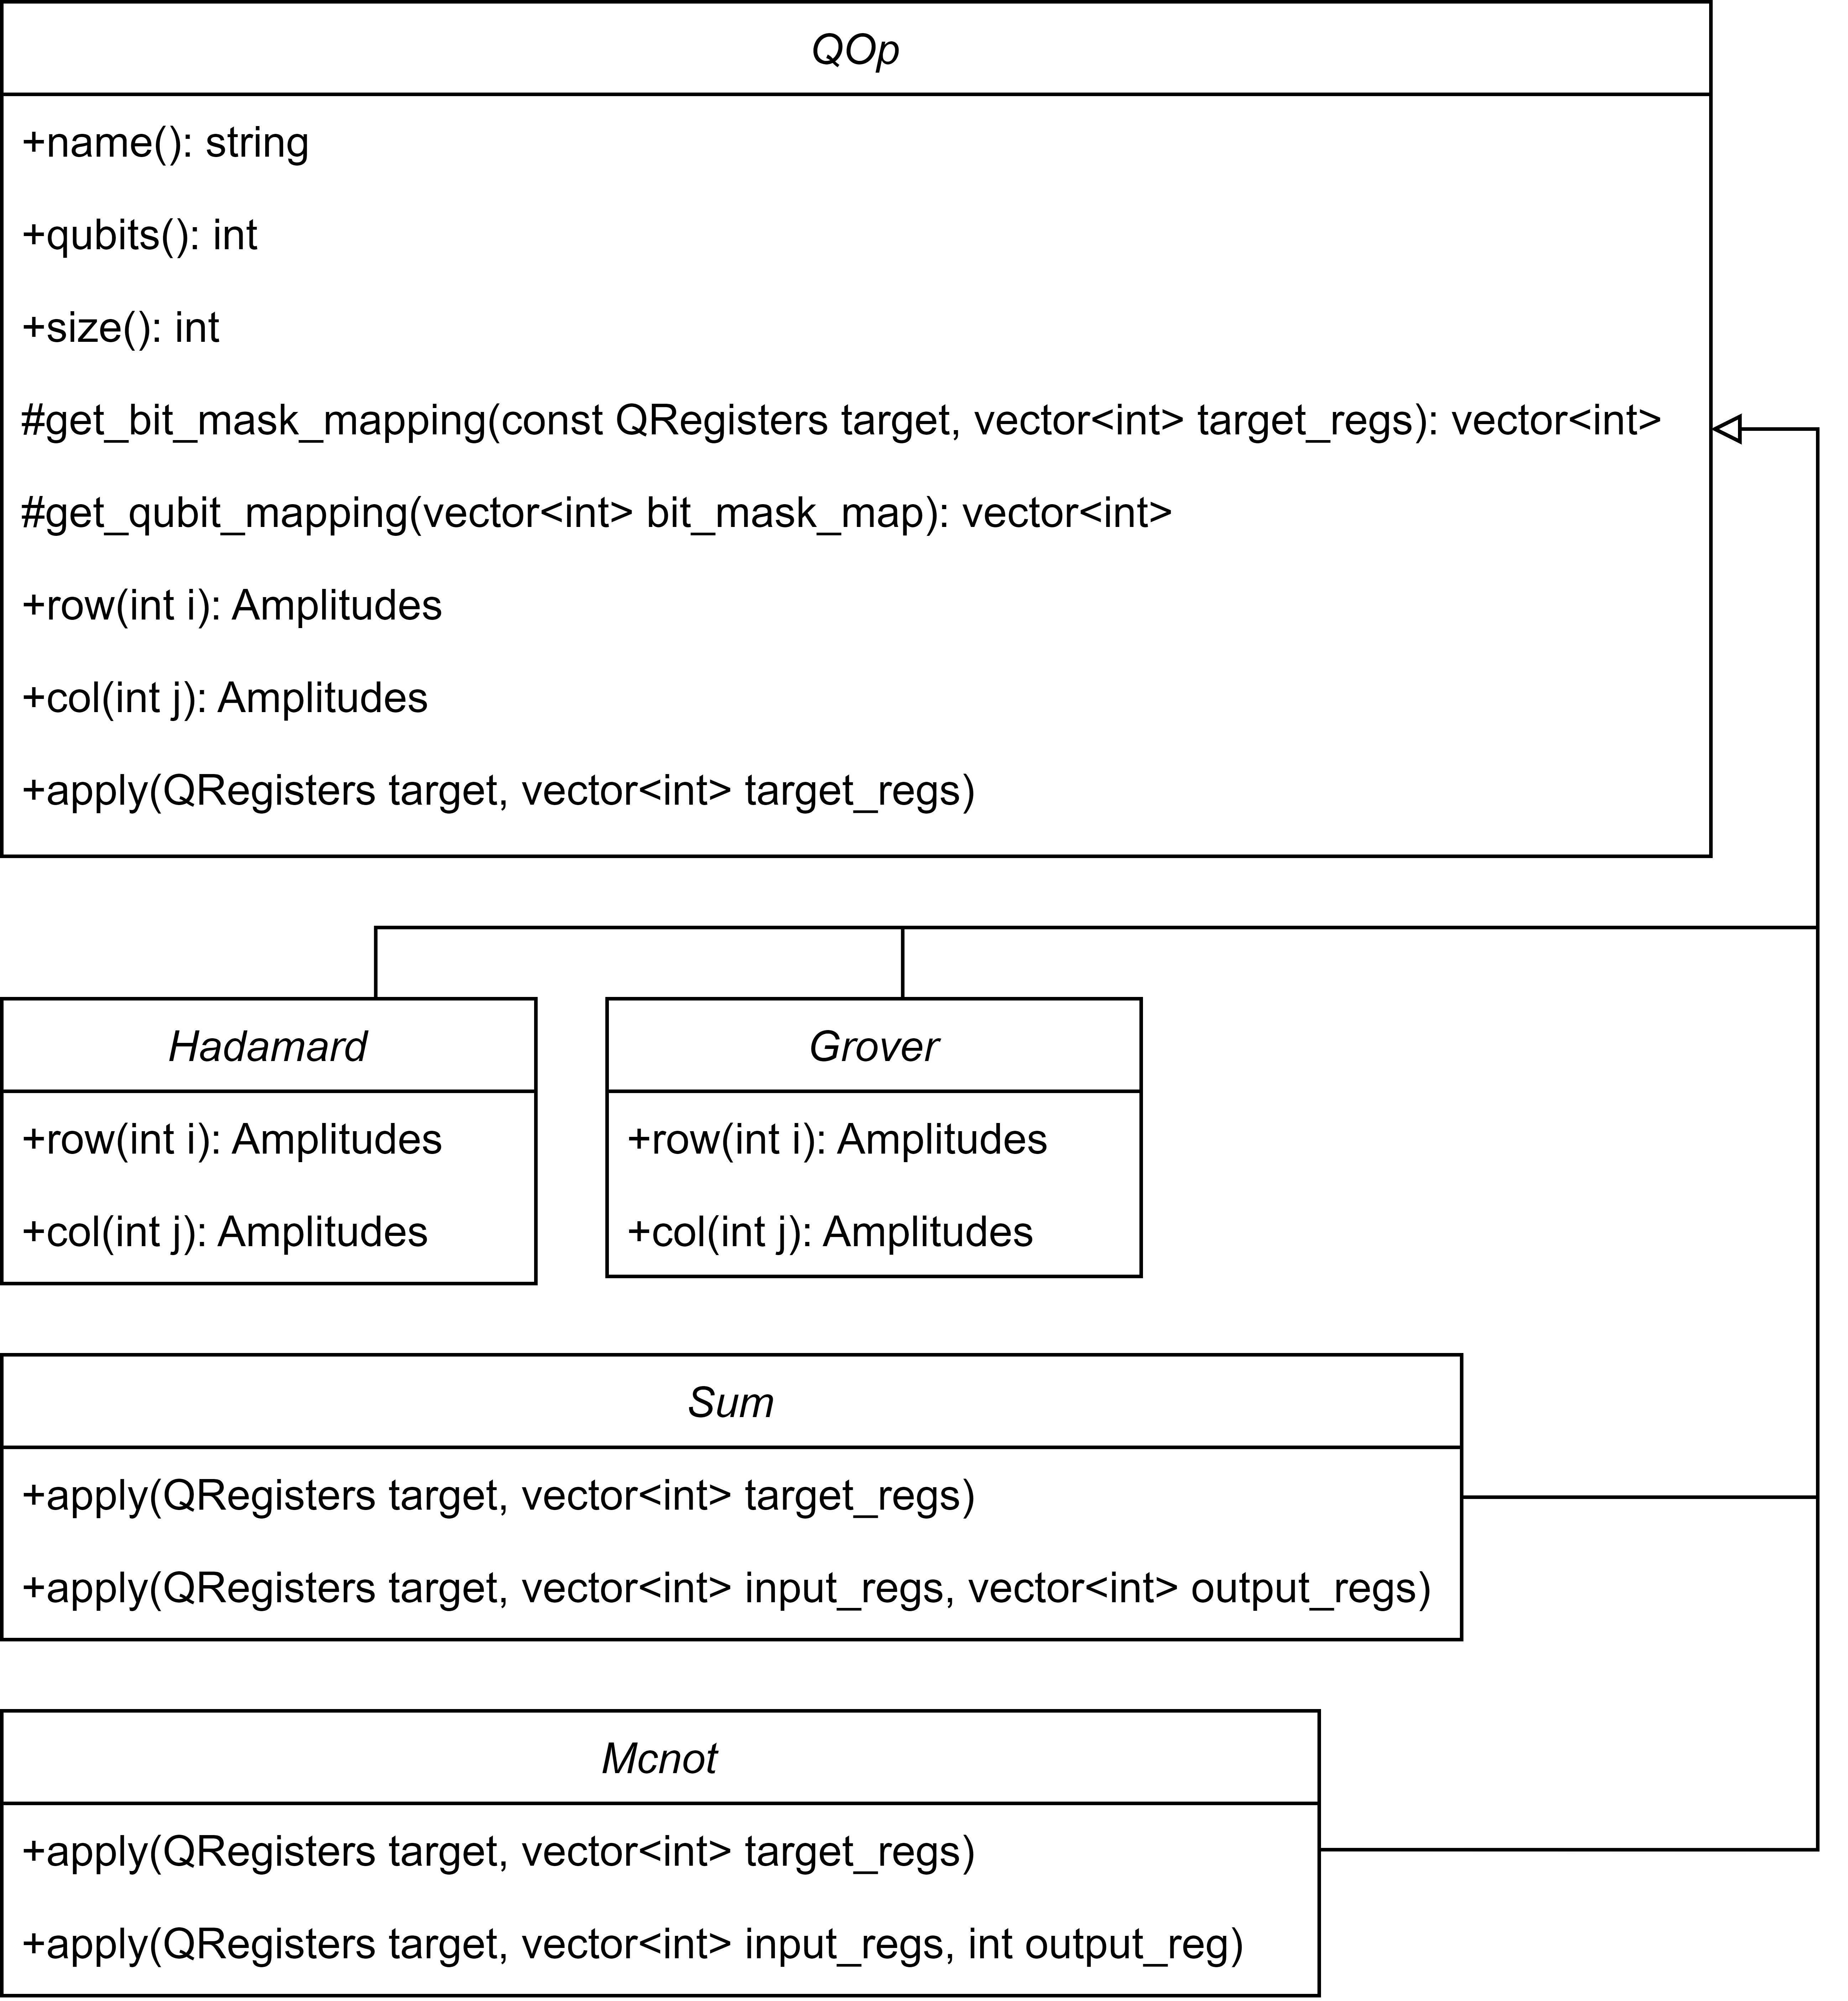
\includegraphics[width=0.7\linewidth]{content/assets/04_simulator_implementation/uml.png}
    \caption{Strategy and Visitor pattern}
\end{figure}

The \texttt{QOp} class is the base class of all of the others. The \texttt{Hadamard}, \texttt{Grover}, \texttt{Sum} and \texttt{Mcnot} classes all inherit from it. In particular, the \texttt{Hadamard} and \texttt{Grover} classes only redefine the \texttt{row} and \texttt{column} methods. The generic implementation of the apply method in \texttt{QOp} then uses these methods to apply the operator on the QRegisters.

The \texttt{get\_bit\_mask\_mapping} and \texttt{get\_qubit\_mapping} methods deal with the probability amplitude permutation and the \textbf{BISM} mapping. They are protected, so inherited classes can make use of them too.

The \texttt{Sum} and \texttt{Mcnot} required me to implement a form of inversion-of-control. In the first iteration, a third class (an \texttt{Orchestrator}) received both the registers and the operator it should apply to them, iteratively generated the necessary rows from the operator and applied them onto the registers. This was poblematic, because this type of control flow made it difficult to implement the \texttt{Sum} and \texttt{Mcnot} operators, since they calculate their result without relying on an explicit representation row format.

The knowledge of how an operator should be applied to the registers should be given to the operator itself, since the framework relies on clever, operator-specific memory-efficient implementations to function. This is exactly what the Visitor pattern is used for. According to the Design Patterns\cite{DesignPatterns} book we can \textit{``Use the Visitor pattern when many distinct and unrelated operations need to be performed on objects in an object structure, and [we] want to avoid "polluting" their classes with these operations. Visitor lets [us] keep related operations together by defining them in one class. When the object structure is shared by many applications, use Visitor to put operations in just those applications that need them.''}
